\section{Simulation kritischer Schaltungsteile}
\subsection{Sendeeinheit}
\subsubsection{Eingangsteil}
Die Eingangskaskade(siehe Abb.\ref{kaskade}) wird in LTSPice simuliert. Zweck dieser Simulation ist die Verifizierung der Schutzfunktion. Die Sendeeinheit wird dabei als kleinerer Widerstand eines Niederspannungsteiler bestehend aus der jeweiligen Impedanz und einem $280M\Omega$. In den Abbildungen \ref{impedanz20k} und \ref{impedanz50k} wird gezeigt ab welcher Quellspannung(Spannung über dem Spannungsteiler) die Eingangsspannung der Sendeeinheit begrenzt wird. Auf der X-Achse ist hierbei die Quellspannung und auf der Y-Achse die Eingangsspannung der Sendeeinheit dargestellt. 
\begin{figure}[H]
\centering
 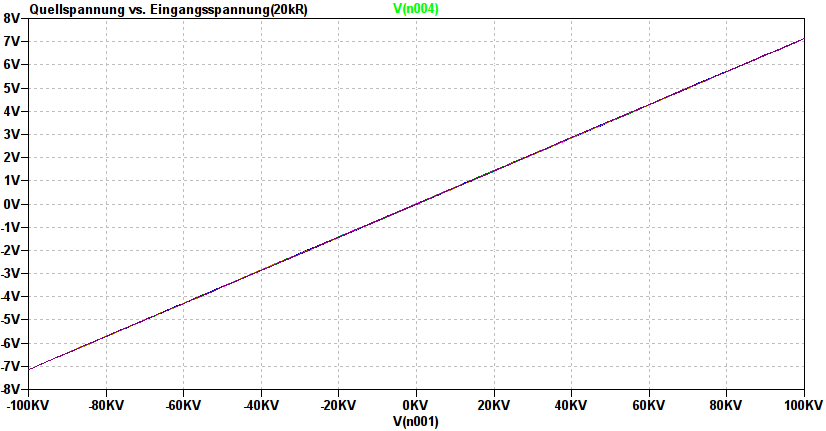
\includegraphics[scale=0.5]{gfx/simTx/Impedance20k.png}
 \caption{Eingansspannung vs. Ausgangsspannung $20k\Omega$ Impedanz}
	\label{impedanz20k} 
\end{figure}


\begin{figure}[H]
\centering
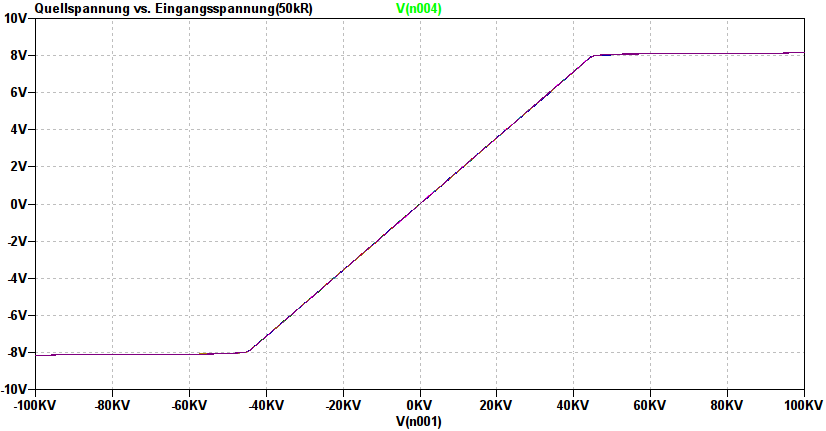
\includegraphics[scale=0.5]{gfx/simTx/Impedance50k.png}
 \caption{Eingansspannung vs. Ausgangsspannung $50k\Omega$ Impedanz}
	\label{impedanz50k} 
\end{figure}


\subsubsection{Millerintegrator}
\label{sec:simMiller}
Zur Verifizierung der PWM Synthese wird der Millerintegrator(Abschnitt \ref{sec:miller}) und der Komparator(Abschnitt \ref{sec:comp}) simuliert. Das obere Diagramm(Abbildung \ref{fig:pwmSynth}) zeigt das Eingangssignal(Sinus,50Hz, $8V_{pp}$) und das Dreieckssignal aus dem Millerintegrator(Dreieck, 1kHz, $10V_{pp}$). Das untere Diagramm zeigt den Ausgang des Komparators und somit die synthetisierte PWM.
\begin{figure}[H]
\centering
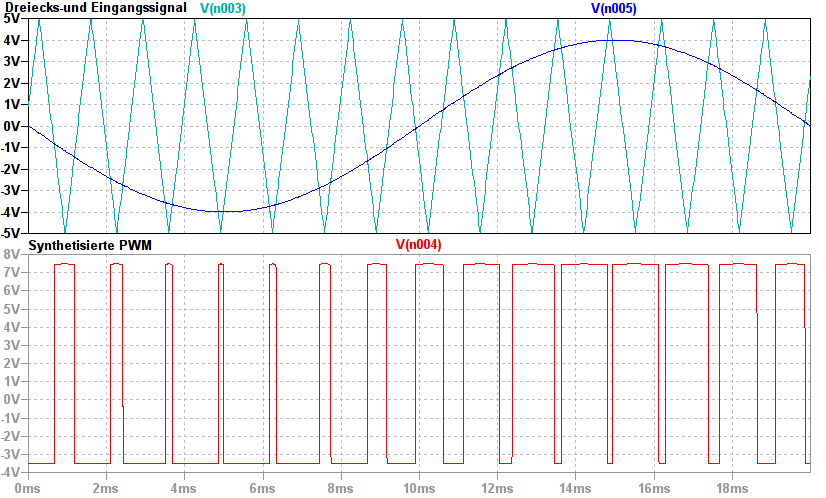
\includegraphics[scale=0.5]{gfx/simTx/PWMsynth.png}
\caption{Simulation Millerintegrator und PWM-Synthese}
	\label{fig:pwmSynth} 
\end{figure}
\subsubsection{Diodentreiber}
Um den maximalen Strom durch die Diode zu verfizieren wurde die Konstantstromquelle(Abschnitt \ref{sec:ksq}) simuliert. In der Simulation wurde der Widerstand $R_9$(siehe Abb.\ref{fig:diodedriver}) mittels Monte-Carlo Simulation von $0 - 100\Omega$ variiert. Das Diagramm zeigt den Strom durch die Sendediode für verschiedene Widerstandswerte.
\begin{figure}[H]
\centering
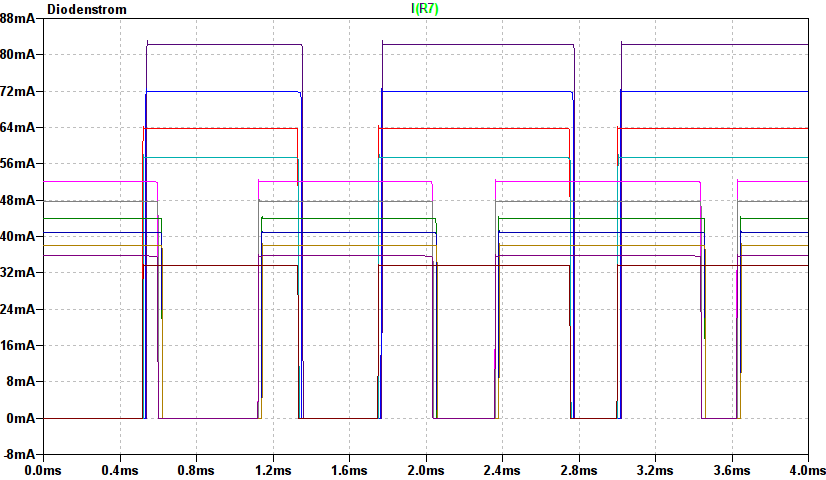
\includegraphics[scale=0.5]{gfx/simTx/DiodeCurrent.png}
\caption{Simulation Diodenstrom}
	\label{fig:pwmSynth} 
\end{figure}

